\chapter{Overview of the LHC and CMS}
\label{chap:detector}
\section{The Large Hadron Collider (LHC)}
\label{sec:lhc}
%The \LHC~\cite{LHC_machine} is a synchrotron of circumference 27\km, currently the largest and most powerful in the world, installed in the tunnel which previously contained the \LEP~\cite{lepdesign} collider at \CERN. 
The \LHC~\cite{LHC_machine} is currently the largest and most powerful synchrotron in the world, and is installed in the tunnel which previously contained the \LEP~\cite{lepdesign} collider at \CERN. 
The tunnel is located roughly 100\m underground near Geneva, on the border between Switzerland and France. The LHC was designed to perform collisions of two types: \pp (proton-proton) collisions and, less frequently, heavy ion collisions, for example \PbPb (lead-lead). The former is used to search for new particles and perform \SM measurements, such as the ones presented in this thesis. The latter is used, for example, for studies of quark-gluon plasma, and is not discussed in detail here. 

The \LHC is the last stage in a series of machines which form the \CERN accelerator complex, which is illustrated in \Fig~\ref{fig:accelerators}. The procedure by which particles are accelerated using this chain of machines is described in~\cite{LHC_machine}, and is summarised below. In \pp collisions, protons are first obtained from a hydrogen gas, which is stripped of electrons. The particles are then brought up to an energy of 50\MeV using \LINACTWO. The particles coming out of the initial linear accelerator are transfered into the \Booster, which raises the beam energy to 1.4\GeV, before the beams enter the \PS. At this stage, the protons energies are increased to 25\GeV. Once the beams reach the required energy, they are passed into the \SPS, and boosted to 450\GeV. Finally, the beams are injected into the LHC rings, which are two concentric beampipes within the same set of bending magnets. The LHC then brings the beams up to their final energy, which, in the most recent run, was approximately 6.5\TeV, leading to a centre-of-mass collision energy of $\sqrt{s}=13\TeV$. A further increase in the beam energy is foreseen in the \LHC programme, which would bring it up to its design value of 7\TeV per beam, and $\sqrt{s}=14\TeV$.

\begin{figure}[h]
\centering
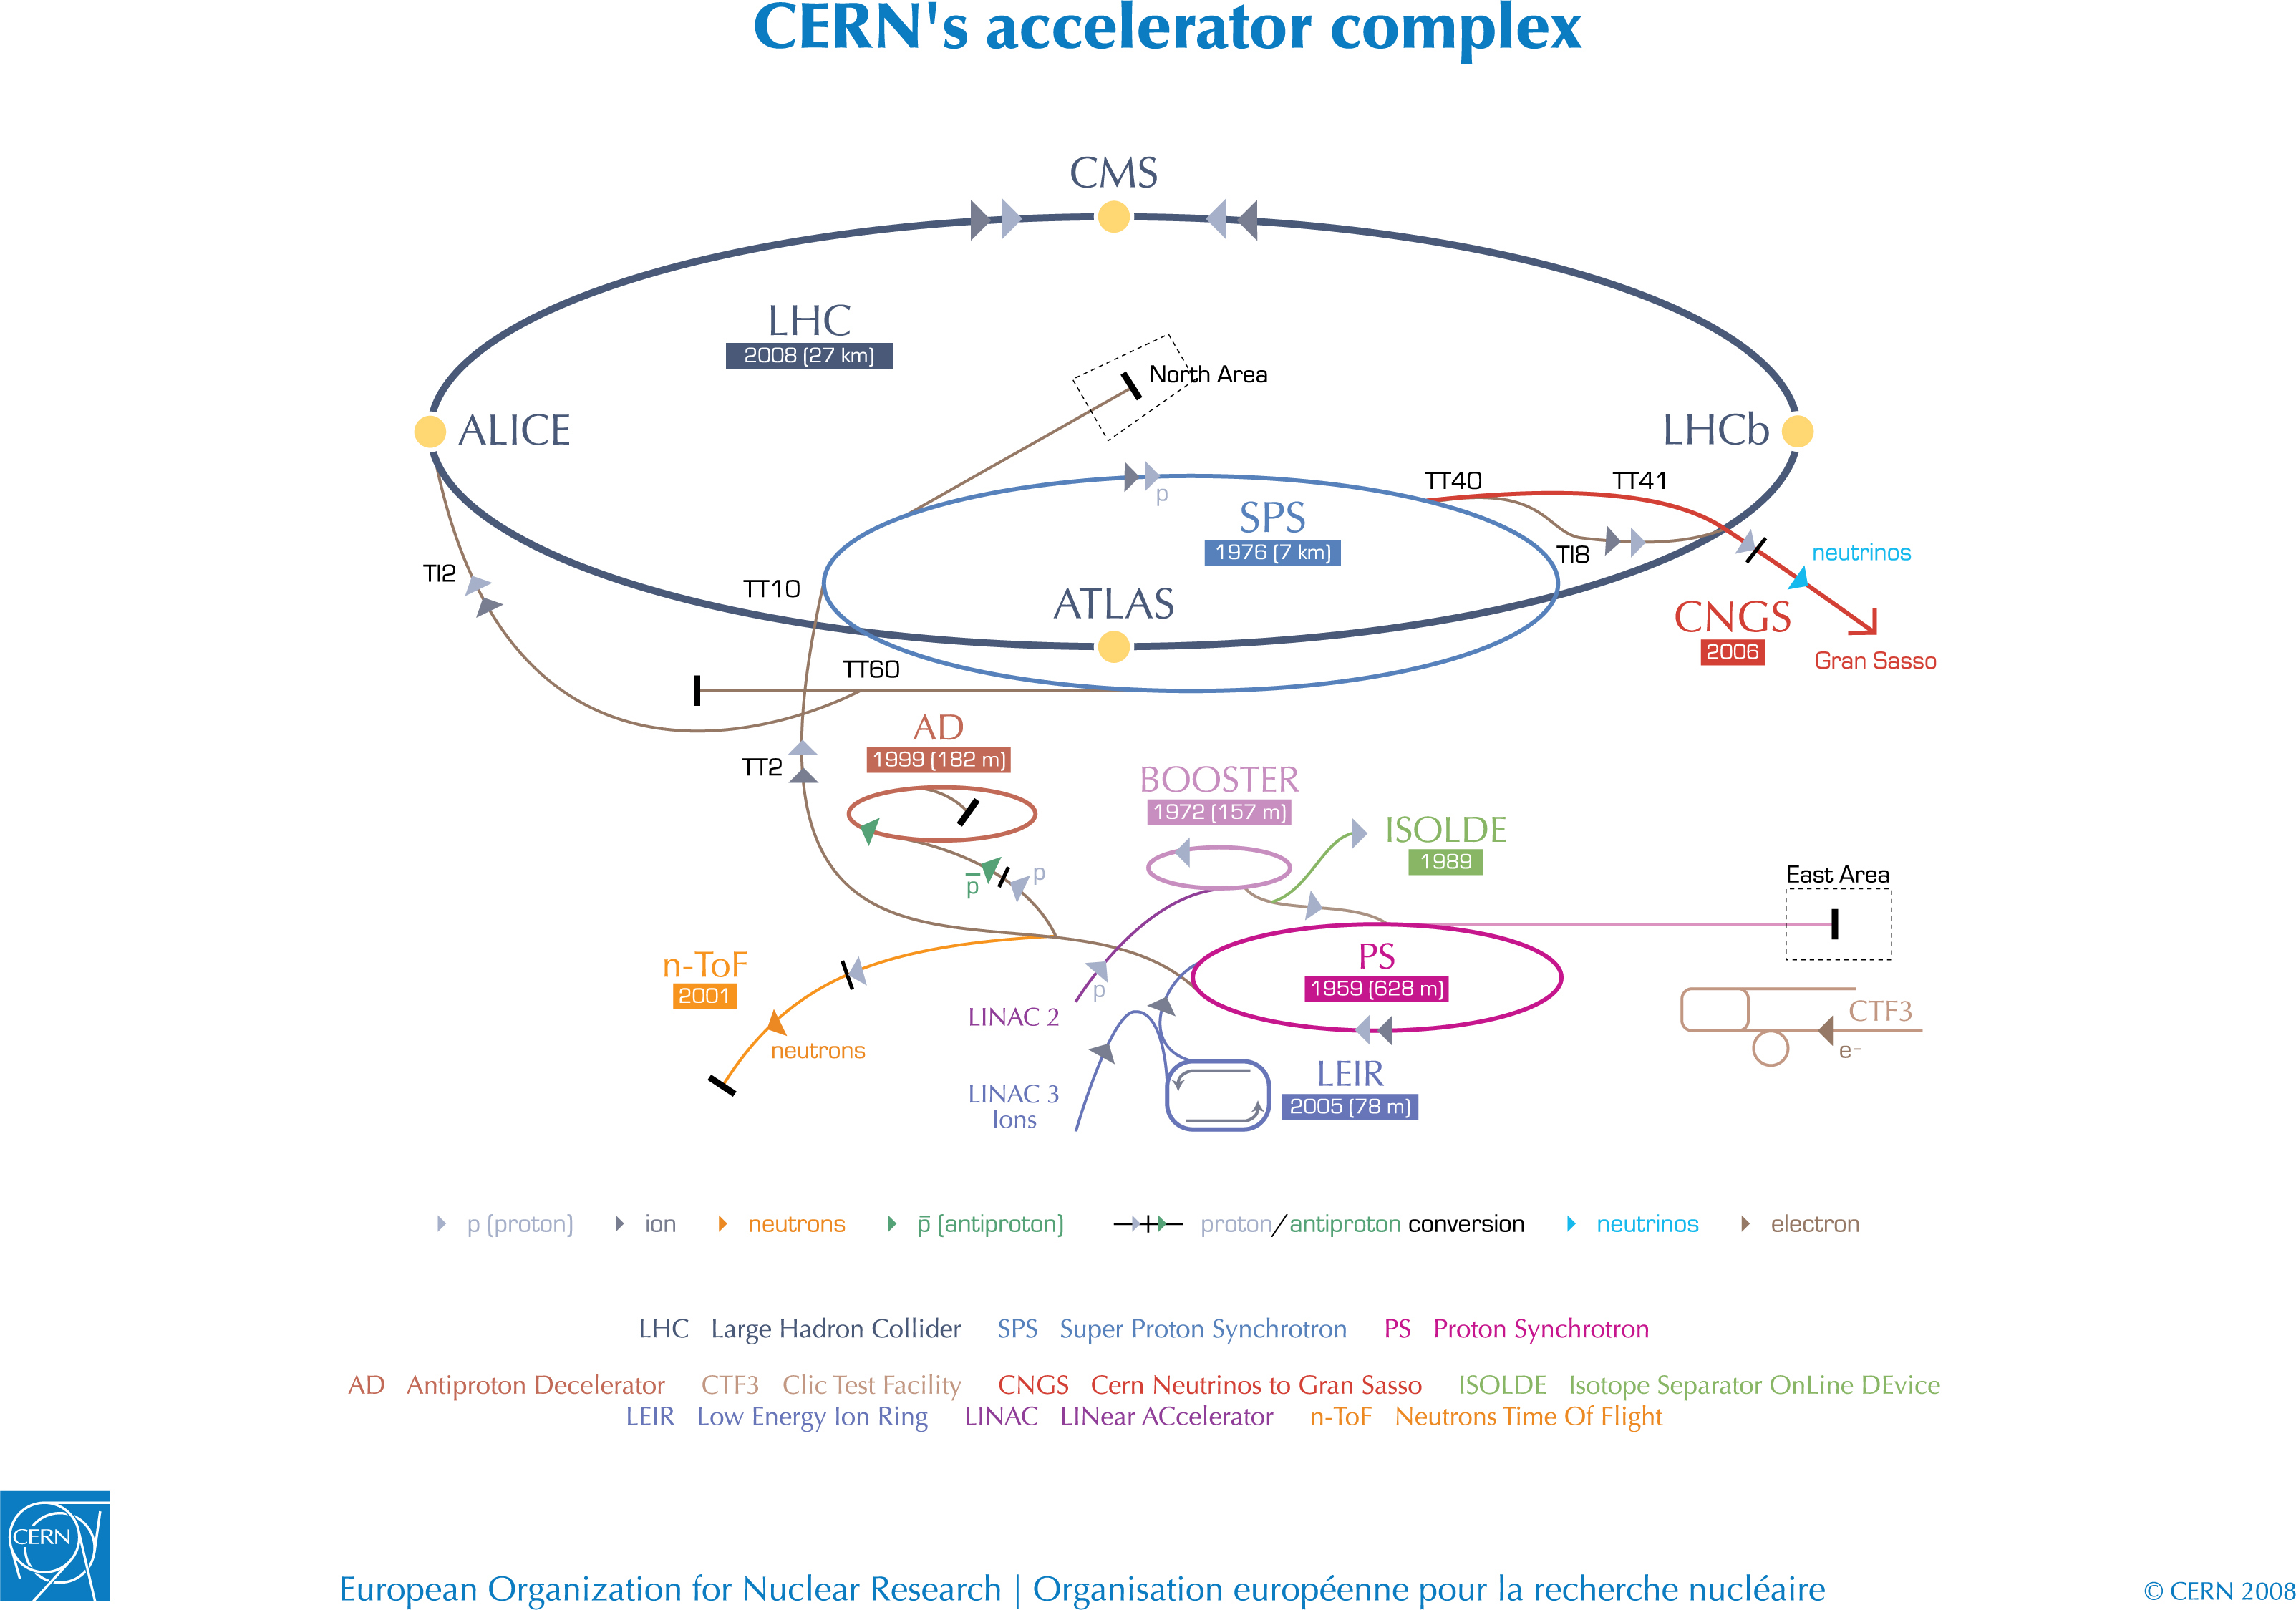
\includegraphics[width=1.0\textwidth]{detectorFigures/accelerators.jpg}
\caption[Schematic view of the CERN accelerator complex, showing the chain of machines which allow the energies of the particles to increase to 6.5\TeV: LINAC2, PS Booster, PS, SPS and finally LHC\quad\cite{Christiane:1260465}.]{Schematic view of the CERN accelerator complex, showing the chain of machines which allow the energies of the particles to increase to 6.5\TeV: LINAC2, PS Booster, PS, SPS and finally LHC~\cite{Christiane:1260465}.}
\label{fig:accelerators}
\end{figure}

The counter-circulating beams in the \LHC are bunched, with each bunch containing several billion protons. The bunch spacing was 50\ns in the initial running of the \LHC, but has now been reduced to its design value of 25\ns, to allow a faster accumulation of data. The average number of times a process occurs in collision experiments ($N_{\text{process}}$) can be obtained from the following relation~\cite{Benedikt:823808}:
\begin{equation}
\label{eq:NeqSigmaL}
N_{\text{process}} = \sigma_{\text{process}}\times \mathcal{L}_{\text{int}},
\end{equation}

where $\sigma_{\text{process}}$ is the \crosssection of the process and $\mathcal{L}_{\text{int}}$ is the integrated luminosity, which is the time integral of the instantaneous luminosity $L$. The luminosity depends only on the machine parameters, and assuming a Gaussian beam distribution, is given by the relation~\cite{Benedikt:823808}:
\begin{equation}
\label{eq:NeqSigmaL}
L = \frac{n_{b} N^{2}_{b} f_{\text{rev}} \gamma_{r}}{4 \pi \epsilon_{n} \beta^{*}} F,
\end{equation}
where $n_{b}$ is the number of bunches in each beam, $N_{b}$ is the number of particles per bunch, $f_{\text{rev}}$ is the revolution frequency, $\gamma_{r}$ is the relativistic gamma factor, $\epsilon_{n}$ is the normalised transverse beam emittance, $\beta^{*}$ is the beta function at the collision point and $F$ is a luminosity reduction factor which takes into account the fact that beams cross at a slight angle. 

The \LHC began operation at $\sqrt{s}=7\TeV$ in 2010, collecting 44\ipb of data in 2010 and 6.1\ifb in 2011. In 2012, the collision energy was successfully increased to $\sqrt{s}=8\TeV$ and 23.3\ifb of data were recorded. This period corresponded to the first physics run of the \LHC (\RunI). After a shutdown period for planned upgrades to the machine, the \LHC began \RunII and raised its collision energy to $\sqrt{s}=13\TeV$, delivering 4.3\ifb in 2015 and \totaldatatwentysixteen\ifb in 2016, as can be seen in \Fig~\ref{fig:totalintlumi}. 
\ifNewAnalysis
The analysis of the full 2016 dataset is presented in this thesis, which amounts to \thisanalysislumi\ifb once the data collection efficiency of \CMS is accounted for.
\else
The analysis of the first \thisanalysislumi\ifb collected in 2016 is presented in this thesis.
\fi
The peak instantaneous luminosity of the \LHC, achieved at the start of periods of colliding beams, is currently around $1.4 \times 10^{34}$\lumiunits, significantly exceeding the design luminosity of $1 \times 10^{34}$\lumiunits. \RunII is scheduled to continue until 2018 before another shutdown for upgrades is envisaged. 

\begin{figure}[h]
\centering
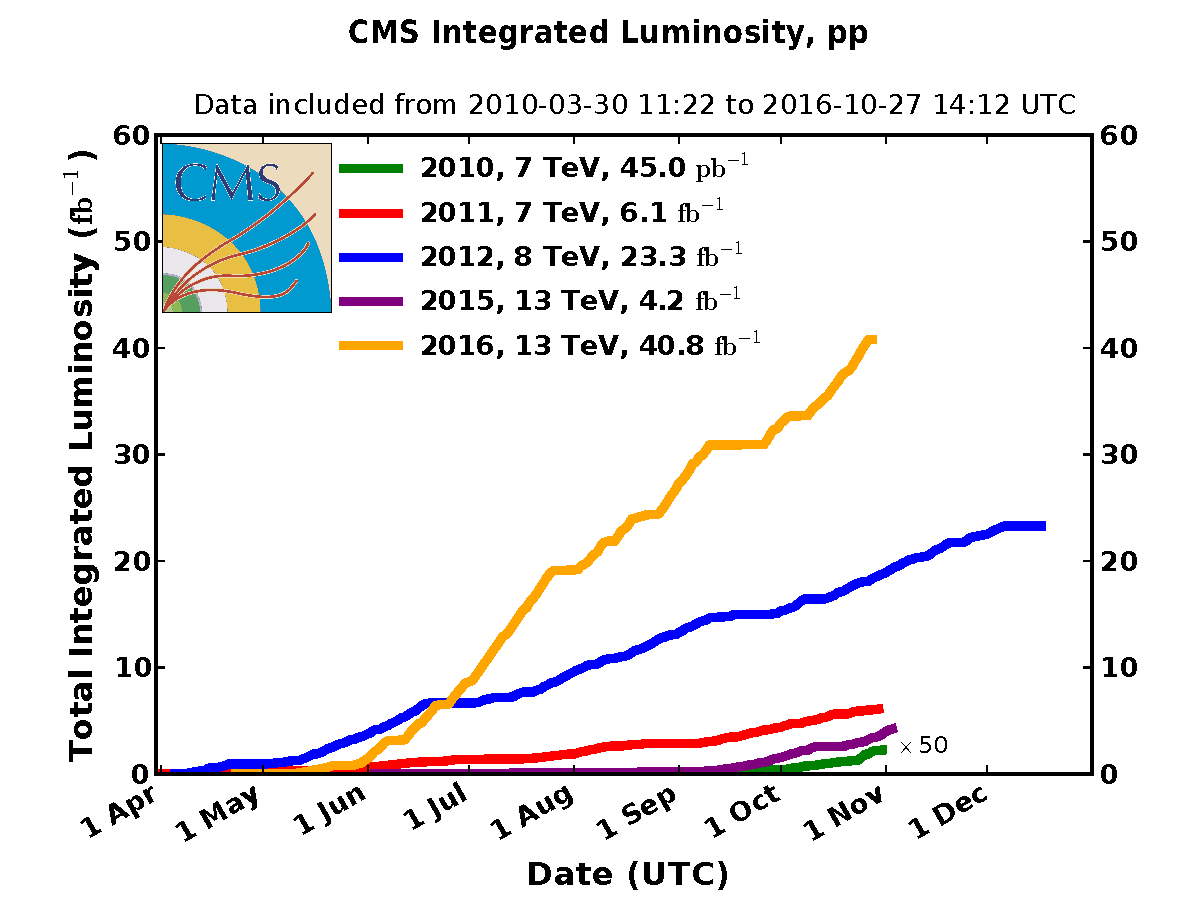
\includegraphics[width=1.0\textwidth]{detectorFigures/int_lumi_cumulative_pp_2_210317.pdf}
\caption[Overview of the integrated luminosity delivered by the LHC throughout its operation until the time of writing, as recorded by CMS\quad\cite{CMSLumiPublic}.]{Overview of the integrated luminosity delivered by the LHC throughout its operation until the time of writing, as recorded by CMS~\cite{CMSLumiPublic}.}
\label{fig:totalintlumi}
\end{figure}

There are eight points along the \LHC ring which are equipped with access shafts, as well as surface and underground structures. Four of these points host \LHC infrastructure elements: the collimators at points 3 and 7, the RF system at point 4 and the beam dump at point 6. The remaining four points house experimental caverns where beams are focused and brought into collision. Two general purpose detectors are located at diametrically opposed sides of the ring: \ATLAS~\cite{AtlasatLHC} at point 1 and \CMS~\cite{CMSatLHC} at point 5. Two additional specialised detectors are located at points 2 and 8, namely \ALICE~\cite{AliceatLHC} (used in the study of heavy ion collisions) and \LHCb~\cite{LHCbatLHC} experiment (specialising in flavour physics), respectively. 



\section{The Compact Muon Solenoid (CMS)}
\label{sec:cms}

\subsection{Overview}
\label{sec:cms:overview}

\CMS is located approximately 100\m underground at access point 5 of the \LHC, near the French village of Cessy. It is over 21\m long and 14\m in diameter, weighing over 12,500 tons. It consists of a superconducting solenoid magnet 13\m long and 5.9\m in diameter, generating a 3.8\T magnetic field, which is embedded within an iron return yoke containing the muon detection system. The other sub-detectors are contained within the solenoid. The layout of the \CMS detector can be seen in \Fig~\ref{fig:cms-exploded}. \CMS is composed of a cylindrical barrel region closed by two endcaps. The tracker (described in \Sec~\ref{sec:cms:tracker}), \ECAL (described in \Sec~\ref{sec:cms:ecal}), and \HCAL (described in \Sec~\ref{sec:cms:hcal}) are housed within the solenoid. Outside of the solenoid, four layers of iron act as a return yoke for the magnet and house muon detector chambers (described in \Sec~\ref{sec:cms:muondetector}). 

The \LHC experiments use a right-handed coordinate system whereby the $x$-axis points towards the centre of the \LHC ring, the $y$-axis points upwards, and the $z$-axis points in the direction of the counter-clockwise beam. A more convenient coordinate system can be defined for physics analyses using the variables $(\eta,\phi,z)$. In this convention, $\eta = -\ln [ \tan(\theta/2)]$ is the pseudorapidity (where $\theta$ is the polar angle relative to the beam axis) and $\phi$ is the angle relative to the $x$-axis in the $(x,y)$ plane. The plane perpendicular to the $z$-axis is referred to as \emph{transverse}, while the direction pointing along it is referred to as \emph{longitudinal}. The transverse components of energy and momentum are denoted by \ET and \pT respectively. 

%Each instance where the data from a bunch crossing are saved by the detector is known as an event. Typically, an event will have a single interaction which is of interest. At 13\TeV the \pp interaction \crosssection is very large, so several interactions per crossing are expected. The physical locations of these interactions are referred to as vertices, with the interaction of interest occurring at the \PV, and other interactions at secondary vertices. The additional interactions in an event, other than the one occurring at the \PV, are collectively referred to as \PU. 

\begin{figure}[h]
\centering
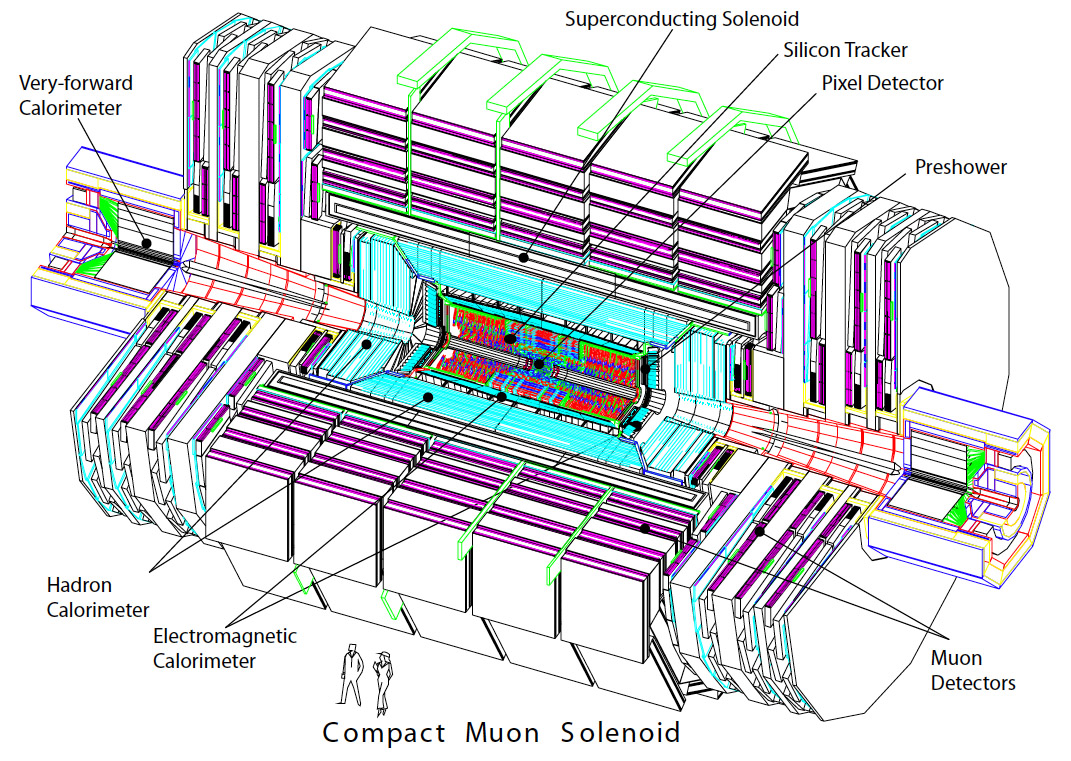
\includegraphics[width=1.0\textwidth]{detectorFigures/cms-perspective.png}
\caption[A cutaway diagram of the CMS detector, showing the main components and \subdetector\s, which are described in \Sec \ref{sec:cms}\quad\cite{CMSTDR}.]{A cutaway diagram of the CMS detector, showing the main components and \subdetector\s, which are described in \Sec~\ref{sec:cms}~\cite{CMSTDR}.}
\label{fig:cms-exploded}
\end{figure}

\subsection{Tracker}
\label{sec:cms:tracker}

The closest \subdetector to the beam crossing point is the tracker~\cite{CMSTrackerTDR}, the layout of which can be seen in \Fig~\ref{fig:trk}. This \subdetector, which fits within a cylindrical volume 5.8\m long and 2.5\m in diameter, is used to measure the momenta of charged particles whose tracks are deflected in the 3.8\T magnetic field. 
The short interval between collisions (25\ns) requires the tracker to have a fast response time. Furthermore, the large \pp \crosssection necessitates it to be resistant to radiation. The two requirements are satisfied by silicon-based detectors. Two silicon detector types are used in the \CMS tracker: the pixel layers and the silicon strip layers.

%The barrel section of the tracker comprises three cylindrical layers of silicon pixel detectors close to the interaction region, surrounded by ten layers of silicon strip detectors. The endcaps consist of two discs of silicon pixel detectors and twelve discs of silicon strip detectors. Momenta of charged particles can be determined by measuring the curvature of tracks as they bend in the strong magnetic field. For tracks of \pT of the order of 100\GeV, the \pT resolution of the tracker is between 1.5\% and 2.5\%. %% repeated information


\begin{figure}[h]
\centering
\includegraphics[width=1.0\textwidth]{detectorFigures/trackerSchematic.png}
\caption[A diagram showing the layout of the CMS tracker components: the pixel tracker (labelled PIXEL) is the nearest to the interaction region marked by the black dot. The various sections of the strip tracker (TIB, TID, TOB, TEC$+$ and TEC$-$) are arranged around the pixel tracker\quad\cite{CMSTDR}.]{A diagram showing the layout of the CMS tracker components: the pixel tracker (labelled PIXEL) is the nearest to the interaction region marked by the black dot. The various sections of the strip tracker (TIB, TID, TOB, TEC$+$ and TEC$-$) are arranged around the pixel tracker~\cite{CMSTDR}.}
\label{fig:trk}
\end{figure}

The pixel layers are made up of 66 million 100\um $\times$ 150\um silicon pixels. As can be seen in \Fig~\ref{fig:trk}, these are arranged into three concentric cylinders in the barrel section (of radii between 4.4\cm and 10.2\cm) and two planes on each endcap. The spatial resolution of this part of the tracker is around 10\um in the transverse direction. The pixel layers also have excellent longitudinal resolution (20-40\um), which is important for vertex reconstruction~\cite{trackerperformance2014}.

The silicon strip layers surround the pixel layers, and are composed of several sections. Four cylindrical layers form the tracker inner barrel (TIB), while the tracker inner disks (TID) are composed of three planes. Surrounding this, the tracker outer barrel (TOB) provides a further 6 cylindrical layers, while 9 planes form the tracker endcaps (TEC). The silicon strip layers extend to 110\cm in radius. This section of the tracker uses 9.3 million strips, with each strip being 10-20\cm long and 80-183\um wide. The transverse spatial resolution of the silicon strip layers is between 13-38\um in the inner section and 18-47\um in the outer section~\cite{trackerperformance2014}.

Charged particles follow helical trajectories in the \CMS magnetic field, and deposit charge as they pass through the silicon sensors. The resulting recorded signals are referred to as hits. Using multiple hits in the pixel and strip detectors, the helical trajectory can be reconstructed. The transverse momentum \pT of charged particles can then be extracted from the curvature of the helix. The \pT resolution is of the order of 2-3\% in the $|\eta|<1.6$ region and up to 11\% for the outer section~\cite{trackerperformance2014}. Using the extrapolation from the fitted track and the longitudinal resolution of the pixel detector, tracks are grouped into common points of origin, at the \PV and secondary vertices. 

\subsection{Electromagnetic Calorimeter}
\label{sec:cms:ecal}

The \ECAL~\cite{CMSTDR,CMSEcalTDR} is the \subdetector whose performance is the most critical to the \Hgg analysis, and its layout, operation and calibration will therefore be described in some detail. 

\subsubsection{ECAL overview}
\label{sec:cms:ecal:overview}

The \ECAL is made up of an array of 61,200 lead tungstate (PbWO$_4$) crystals in the barrel section and 14,648 crystals in the endcaps, arranged one crystal deep. The choice of material was made because PbWO$_4$ has a short radiation length (the mean distance over which an electron loses all but $1/e$ of its energy to bremsstrahlung) of 0.89\cm. The short radiation length is important in the \ECAL design because it allows electromagnetic showers to be contained within a relatively small depth of material. 
%and a small Moli\`ere radius (the radius of a cylinder containing on average 90\% of a shower's energy) of 1.96\cm. It is also a fast scintillator and radiation resistant. These crystal properties are a central feature of the \CMS detector as it allows excellent energy resolution of incoming photons. 

The \ECAL crystal front faces are 22\mm $\times$ 22\mm squares, corresponding to approximately $\Delta \eta \times \Delta \phi = 0.0174 \times 0.0174$, roughly matching the Moli\`ere radius of PbWO$_4$. The individual crystal depth is approximately 26 radiation lengths, to ensure that the electromagnetic showers are fully contained within the \ECAL. The array of crystals extends to $|\eta| = 3$, but precision measurements are only made up to $|\eta| =2.5$. There are also transition regions between the ECAL barrel and endcaps around $|\eta| = 1.5$. The arrangement of the crystals in the \ECAL can be seen in \Fig~\ref{fig:ecal}.

\begin{figure}[h]
\centering
\includegraphics[width=1.0\textwidth]{detectorFigures/ecalEBEE.png}
\caption[Schematic \crosssection of one quadrant of the ECAL, showing the arrangement of crystals in the ECAL barrel and endcaps. The shower detector (SE, referred to as ES in the text) is also visible, as is the hadron calorimeter barrel (HB) and the tracker (TK)\quad\cite{CMSEcalTDR}.]{Schematic \crosssection of one quadrant of the ECAL, showing the arrangement of crystals in the ECAL barrel and endcaps. The shower detector (SE, referred to as ES in the text) is also visible, as is the hadron calorimeter barrel (HB) and the tracker (TK)~\cite{CMSEcalTDR}.}
\label{fig:ecal}
\end{figure}


%Radiation exposure at the level expected at the LHC does not affect the scintillation mechanism of the crystals.




%\begin{figure}[h]
% \centering
%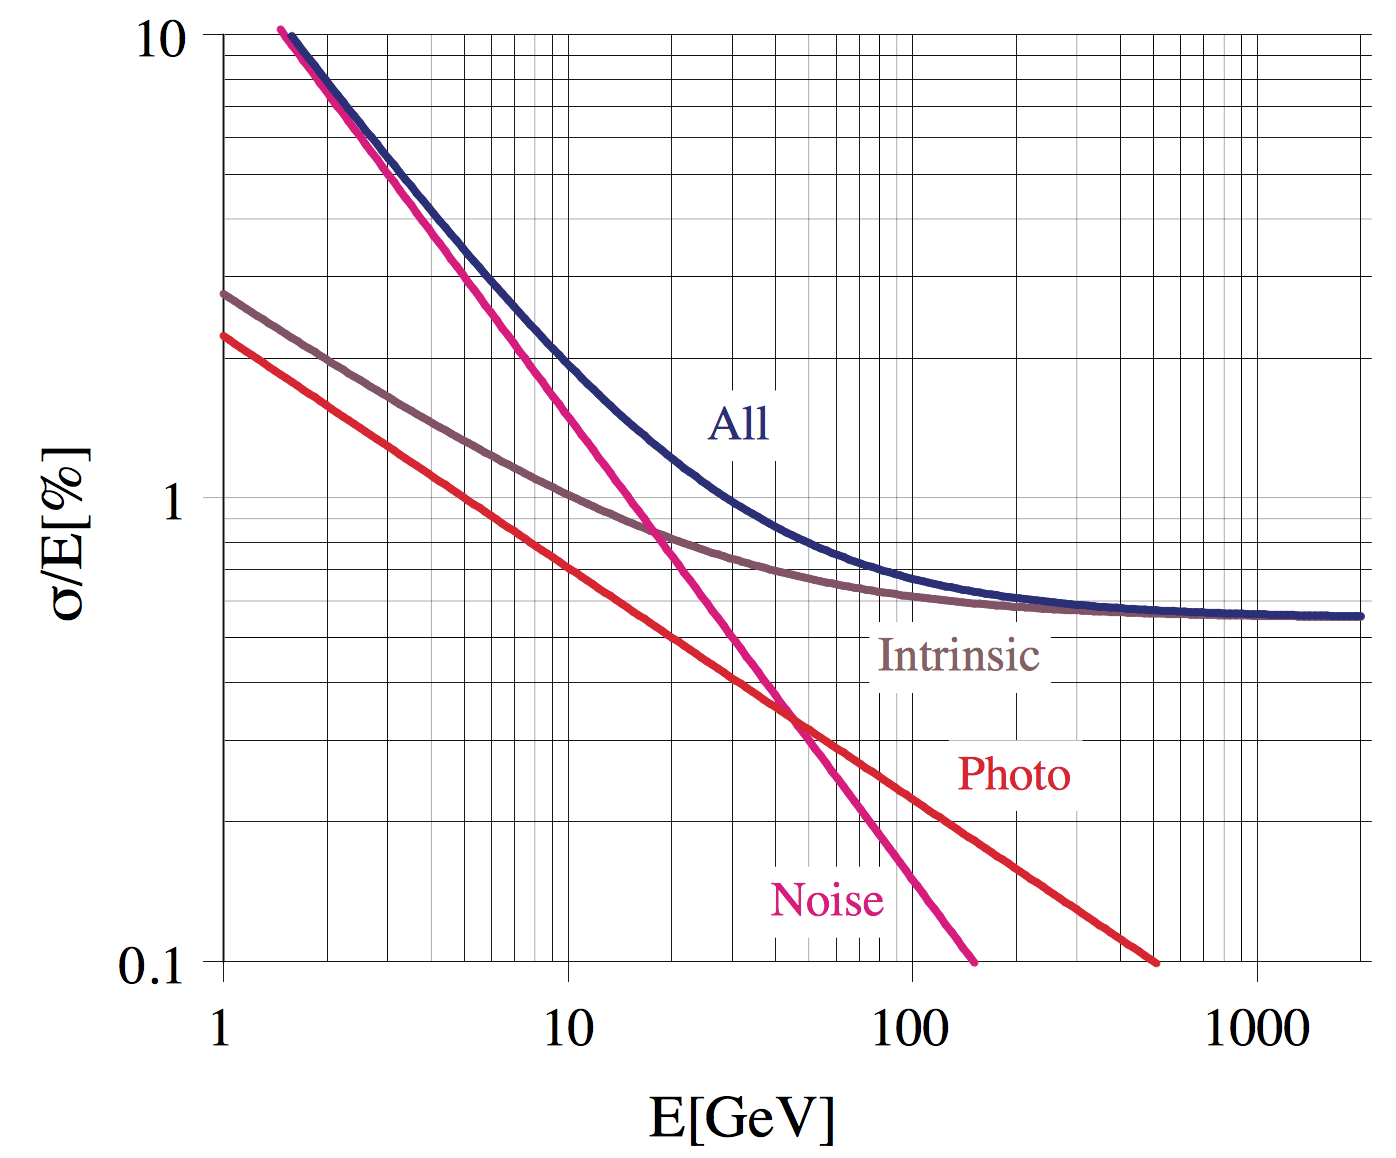
\includegraphics[width=0.6\textwidth]{detectorFigures/EcalResolutionParametrisation.png}
% \caption{The different contributions to the ECAL energy resolution The blue line represents the sum of the stochastic term (red line), the noise term (pink line) and the constant term plus corrected for shower containment (violet line).~\cite{CMSEcalTDR}}
%\label{fig:ecal:resol}
%\end{figure}


The \ECAL consists of the \EB and the \EE. The \EB provides coverage in the region $|\eta| < 1.479$, while the \EE provides coverage for $1.556 < |\eta| < 2.5$. The crystals in the \EB are grouped into 36 supermodules, each covering an angle of $20^o$ in $\phi$. The crystals are arranged so that they do not point directly at the mean position of the primary interaction vertex, but are instead positioned with a $3^o$ offset in both $\theta$ and $\phi$, to help improve the hermeticity of the detector. The \EE is composed of two ``D''-shaped sections, built up of \emph{supercrystals} (units of 25 standard crystals). The \EE has notably worse resolution that the \EB, and this is because the calibration of the crystals is more challenging. One factor contributing to this is that the crystal transparency is affected by the high radiation doses in the \EE. %Another is that the crystal faces in units of $\eta,\phi$ are larger in the \EE than the \EB, and since the energy deposited by additional interactions in a collision, \PU, is roughly constant in unit areas of $\eta,\phi$, the \EE crystals have to deal with more noise.

An additional detector, the \ES, is mounted in front of each endcap, covering the region $1.54 <|\eta| < 2.61$. The main purpose of the \ES is to distinguish between $\pi^0$ and $\gamma$ particles, and also adds three radiation lengths to the depth of the \ECAL endcaps. The \ES is composed of two planes of lead, of 2 and 1 radiation lengths respectively, with high granularity silicon detector strips after each. %The \ES is used to identify $\pi^0\rightarrow \gamma \gamma$ photons, where both photons strike the same crystal. This is possible because the \ES has a much finer granularity than the \EE, so a prompt photon will register in just one strip of the \ES, while a pion decaying to two photons registers in two strips. Although the \EE might interpret $\pi^0\rightarrow \gamma \gamma$ as one highly energetic photon, the high granularity of the silicon strips in the \ES allow two tracks to be identified. 

In the barrel region, \APDs operating with a gain of 50, are attached to the back of the crystals, where the scintillation light is collected. In the endcaps, \VPTs are used instead of \APDs as the photo-detectors. In both cases, the photo-detectors register $\sim 4000 $ photoelectrons per \GeV. The photo-detectors are read out by 12-bit \ADC. Ten consecutive samples are read out and stored for each crystal, and this information is used to determine the amplitude of the pulse, and therefore the amount of energy deposited in the crystal.

The resolution of the \ECAL crystals is modelled with the following equation:
\begin{equation} 
\left( \frac{\sigma}{E}\right) ^2= \left( \frac{S}{\sqrt{E}} \right)^2 + \left( \frac{N}{E} \right)^2 + C^2,
\end{equation}
where $S$ represents the stochastic term, $N$ represents the noise term and $C$ represents a constant term~\cite{CMSTDR}. The design values of these parameters are approximately $S=2.8\%\GeV^\frac{1}{2}$, $ N= 0.12\GeV$ and $C=0.3 \%$. 

As can be seen in \Fig~\ref{fig:det:energy_resol}, for individual \Hgg photons in \RunI, an energy resolution of about 1\% was achieved for unconverted photons in the barrel, and about 2.5\% in the endcaps. For converted photons, an energy resolution of about 1.3\% was observed up to $|\eta| = 1$, rising to about 2.5\% at $|\eta| = 1.4$, and 3-4\% in the endcaps~\cite{CMS-PAS-EGM-14-001}.

\begin{figure}[h]
\centering
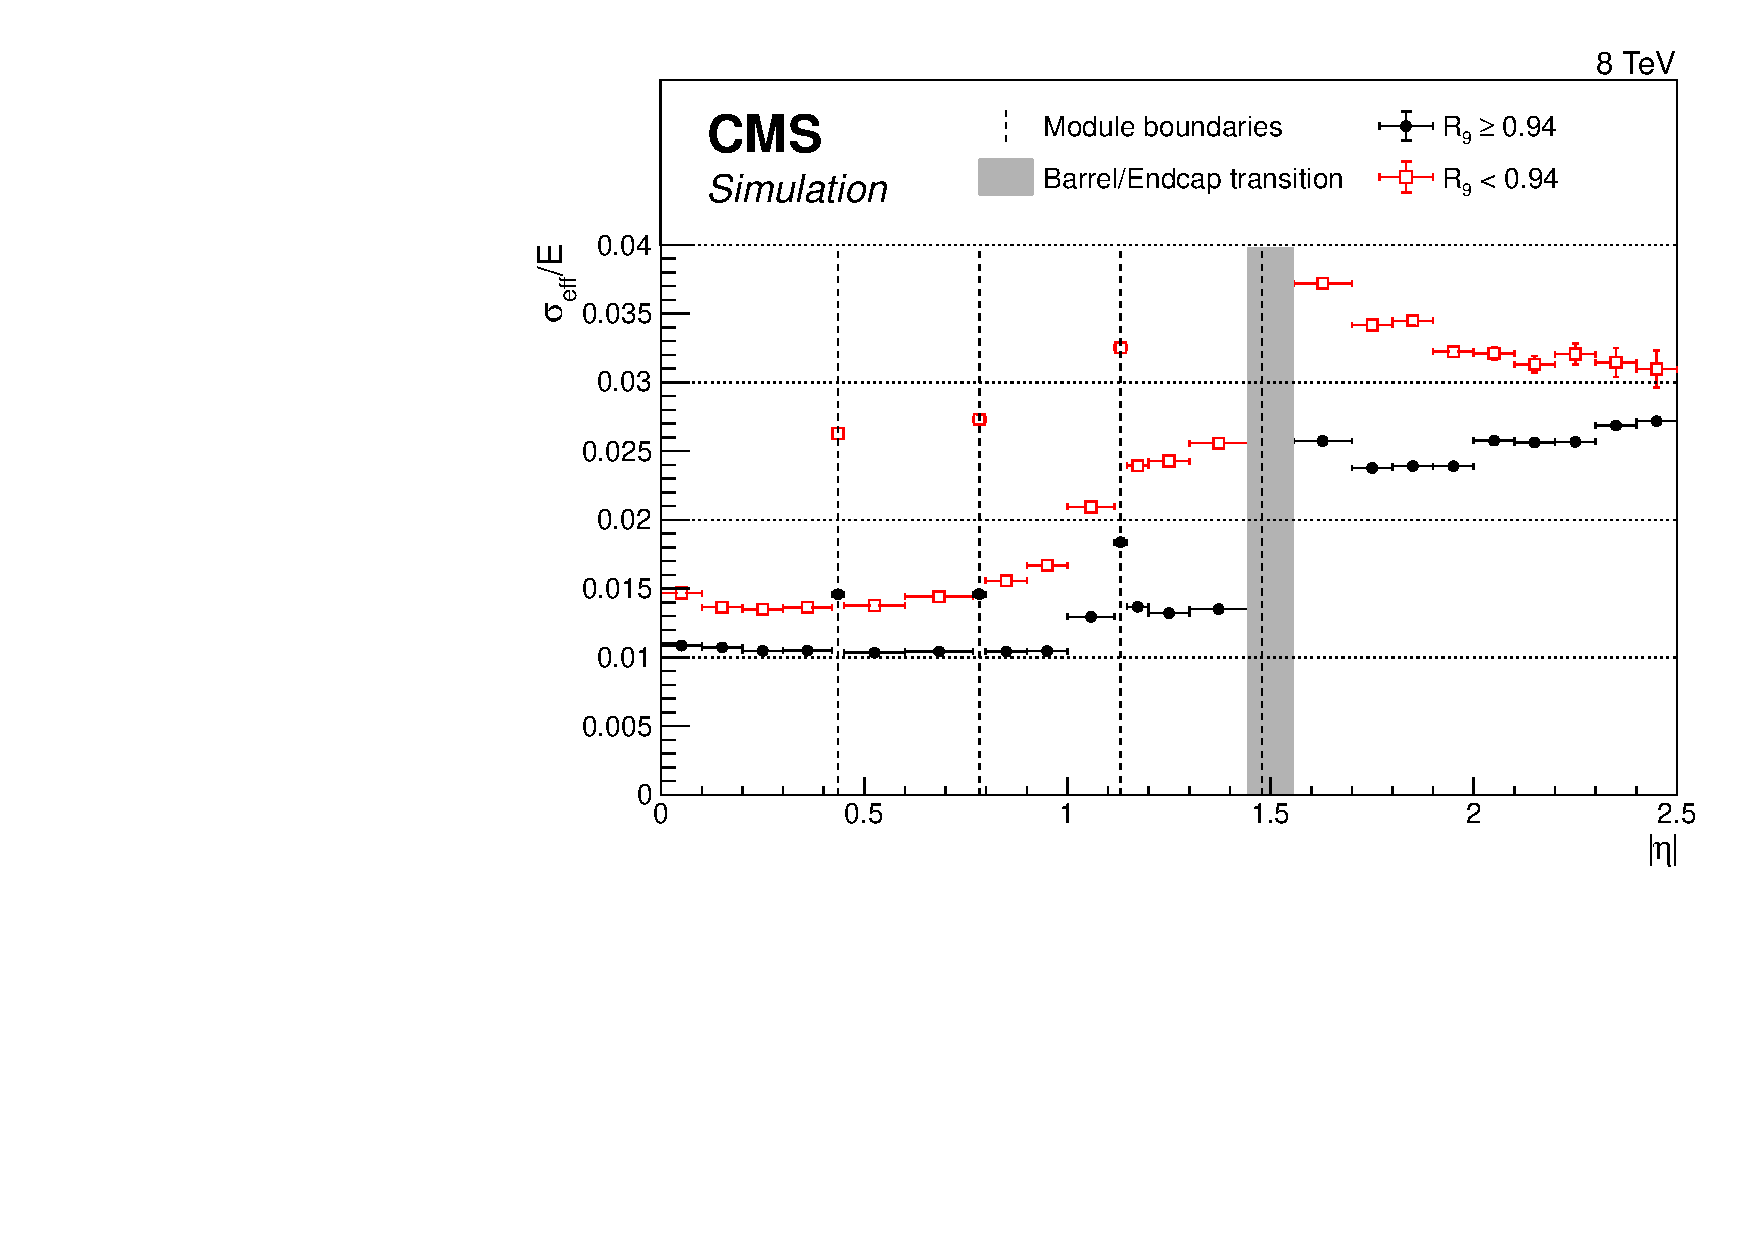
\includegraphics[width=0.8\textwidth]{detectorFigures/effSigma_vs_Eta_mva.pdf}
\caption[The relative energy resolution of individual simulated \Hgg photons in \RunI as a function of $|\eta|$, shown separately for converted photons (black circles) and unconverted photons (open red squares). The vertical lines represent the boundaries between the ECAL modules in the barrel, while the grey band indicates the transition region between the EB and the EE, where photons are not reconstructed\quad\cite{CMS-PAS-EGM-14-001}.]{The relative energy resolution of individual simulated \Hgg photons in \RunI as a function of $|\eta|$, shown separately for converted photons (black circles) and unconverted photons (open red squares). The vertical lines represent the boundaries between the ECAL modules in the barrel, while the grey band indicates the transition region between the EB and the EE, where photons are not reconstructed~\cite{CMS-PAS-EGM-14-001}.}
\label{fig:det:energy_resol}
\end{figure}

\subsubsection{Energy measurement}
\label{sec:cms:ecal:energymeasurement}

Typically, energy deposits will not be contained in a single crystal. When an electron or a photon hits the \ECAL, the electromagnetic shower will spread out into adjoining crystals. In addition, particles can undergo pair conversion or emit bremsstrahlung before impacting the detector, resulting in additional associated energy deposits.
%photons travelling towards the \ECAL can interact with the tracker material and undergo pair conversion, resulting in two nearby or overlapping showers. Furthermore, electrons or positrons travelling towards the \ECAL will be deflected in the $\phi$-direction by the magnetic field, and will emit photons via bremsstrahlung: in this case the radiated photons will make subsequent deposits in the \ECAL. 
Clustering algorithms are used to recover the deposits from the main impact crystal, adjacent crystals where the energy from the main shower is spread out, and the additional associated crystals, and group them into a so-called \SC. %The algorithm by which this is achieved is described in \Sec~\ref{sec:obj:egamma:clustering}. 
The energy of the \SC ($E_{\textrm{SC}}$) can roughly be expressed as: 
\begin{equation} 
\label{eq:cms:ecal:energy}
E_{\text{SC}} = F_{\text{SC}} \cdot G \cdot \Sigma^{i=0}_{N_\text{crystals}}  C_{i} \cdot S_{i}(t) \cdot A_{i} ,
\end{equation}
where $N_\text{crystals}$ is the number of crystals in the \SC, $F_{\text{SC}}$ is a correction to the \SC energy sum representing second-order effects, $G$ is an ADC-to-GeV conversion factor which represents the global energy scale, $C_{i}$ is a factor applied to crystal $i$ to equalise the response (also known as an intercalibration constant), $S_{i}(t)$ is a time-dependent factor to correct for loss of transparency of the crystals, and $A_{i}$ is the amplitude of the pulse recorded in that crystal for the bunch crossing in question. In regions covered by the \ES, the signals from this \subdetector are also used~\cite{cmsEcalCalibration}.


\subsubsection{Calibration}
\label{sec:cms:ecal:calibration}

The calibration of the \ECAL involves using various techniques and physics objects to tune the values of $S_{i}(t)$, $C_{i}$ and $G$ in \Eq~\ref{eq:cms:ecal:energy}. The first step is to make a time-dependent correction for the transparency in the crystals. Indeed, the response of \ECAL crystals varies because of radiation-induced transparency loss and recovery through spontaneous annealing. Continuous monitoring and correction of the response of the crystals is required. This is achieved using a laser which periodically (every 40 minutes) injects photons of wavelength 440\nm into each crystal via a network of optical fibres. The change of the response as measured and corrected for using this mechanism is tracked in \Fig~\ref{fig:cms:ecal:lasercorrections}. The effect of the corrections on the measured mass of the $\pi^0$ in its decay to photons can be seen in \Fig~\ref{fig:cms:ecal:pizeroLMcorr}.


\begin{figure}[h]
\centering
\includegraphics[width=1.0\textwidth]{detectorFigures/EcalLaserCorrections_2.pdf}
\caption[The response of the CMS ECAL lead tungstate crystals is shown as a function of time, and for different pseudorapidity ranges. The crystal response decreases as data are collected, due to transparency loss caused by exposure to radiation, and recovers during spontaneous annealing at times when no beams are present\quad\cite{CMSECALPublic}.]{The response of the CMS ECAL lead tungstate crystals is shown as a function of time, and for different pseudorapidity ranges. The crystal response decreases as data are collected, due to transparency loss caused by exposure to radiation, and recovers during spontaneous annealing at times when no beams are presented~\cite{CMSECALPublic}.}
\label{fig:cms:ecal:lasercorrections}
\end{figure}

\begin{figure}[h]
\centering
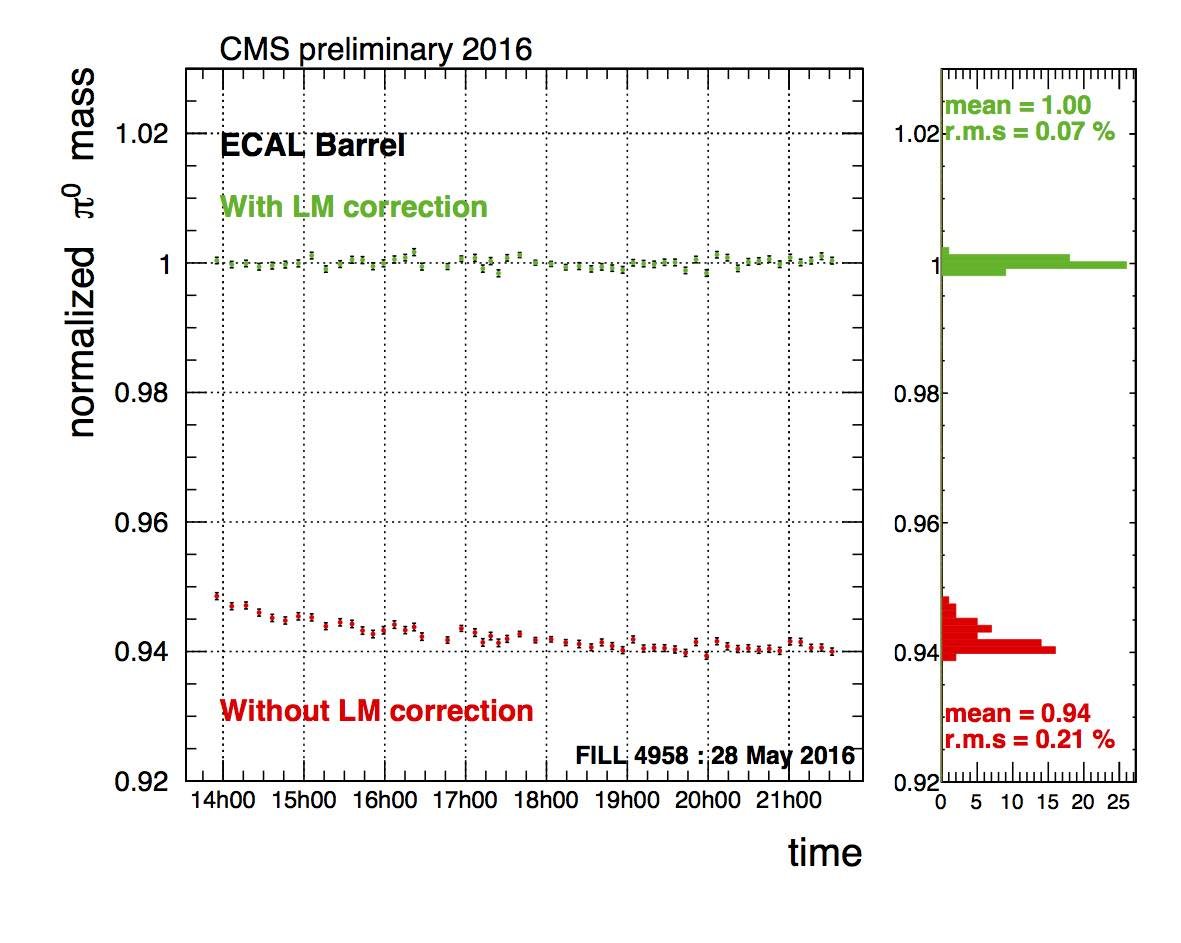
\includegraphics[width=1.0\textwidth]{detectorFigures/pi0_EB_plus_1.jpg}
\caption[The normalised value of the invariant mass of the $\pi^0$ particle in its decay to photons, as measured by the CMS ECAL barrel, with and without the Laser Monitoring (LM) corrections for crystal transparency loss. This example, from a period of less than one day, shows the degradation of the response of the lead tungstate crystals, even over a period of hours\quad\cite{CMSECALPublic}.]{The normalised value of the invariant mass of the $\pi^0$ particle in its decay to photons, as measured by the CMS ECAL barrel, with and without the Laser Monitoring (LM) corrections for crystal transparency loss. This example, from a period of less than one day, shows the degradation of the response of the lead tungstate crystals, even over a period of hours~\cite{CMSECALPublic}.}
\label{fig:cms:ecal:pizeroLMcorr}
\end{figure}

The next step is the intercalibration, which aims to equalise the response of all crystals. This is achieved by determining a set of intercalibration constants $C_{i}$, one for each crystal. Several methods are used in this procedure. The first is to use the fact that the \CMS \ECAL is cylindrically symmetric. It is therefore expected that during a given period of time, the total energy measured by each crystal with the same value of $\eta$ ($\eta$-ring) should be the same. Exploiting the $\phi$-symmetry of the detector, one can therefore produce an intercalibration constant for each crystal in an $\eta$-ring by dividing the amount of energy that was measured by that crystal in an interval of time by the average amount measured by all crystals in that $\eta$-ring. Another method exploits the fact that the invariant mass of $\pi^0$ or $\eta$ particles (as measured in their decay to photons) should be measured the same regardless of the crystal location. Therefore, one can generate intercalibration constants for each crystal by fitting the invariant mass distribution of candidate $\pi^0$ or $\eta$ events where one of the decay photons is centered on the crystal of interest. A correction is applied such that the measured invariant mass agrees with the accepted value. Since the corrections for each crystal depend on the calibration of the other crystals, the procedure is repeated iteratively until a predetermined threshold on the calibration precision is reached.

Intercalibration constants produced using different methods are combined to give a final set of per-crystal corrections. By construction, the average value of the intercalibration constants is unity: these corrections leave the overall scale unchanged.

The final step in the calibration procedure is to set the global scale $G$, which is also the ADC-to-GeV conversion factor. This is set by comparing the measured value of the mass of the $\PZ$ boson in its decay to electrons to the nominal value. Since the mass of the $\PZ$ is well known and simulated, one can set the value $G$ such that the peak of the $\PZ$ invariant mass distribution coincides with the simulated value, in different bins of $\eta$ and \SC type, in order to complete the calibration.


\subsection{Hadronic Calorimeter}
\label{sec:cms:hcal}

The \HCAL is used to identify hadrons, and measure their positions and energies. In particular, it is needed to measure the energy of neutral hadrons which do not leave any hits in the tracker or any deposits in the \ECAL. Such particles need to be taken into account to accurately estimate the energies and directions of jets of particles, and to measure the magnitude and direction of any missing energy, which would indicate particles which did not interact by the \CMS detector (e.g.~neutrinos, or undiscovered weakly interacting particles). 

The \CMS \HCAL is a sampling calorimeter, consisting of active material between absorber plates. The layout of the detector can be seed in \Fig~\ref{fig:hcal}. The active material is a plastic scintillator read out by wavelength-shifting plastic fibres. The absorber plates are made of brass (or steel in the forward section). Brass is chosen as it is an non-magnetic material, and thus will not be affected by the strong magnetic field within the solenoid. The main body of the \HCAL is composed of the \HB with coverage up to $|\eta| < 1.3$, and the \HE with coverage up to $|\eta| < 3$, with $\Delta\phi \times \Delta\eta$ granularities between $0.087 \times 0.087$ and $ 0.17 \times 0.17$. In order to accurately measure missing energy, the \HCAL must be as hermetic as possible. For this reason, an additional calorimeter is appended, the \HF, which gives coverage up to $|\eta| <5$. This uses active quartz fibres within a steel absorber matrix. In order to fully contain hadronic showers, an additional component, the \HO, uses the solenoid as an absorber and is placed directly around it in the barrel region~\cite{cmsHcal}. 

\begin{figure}[h]
\centering
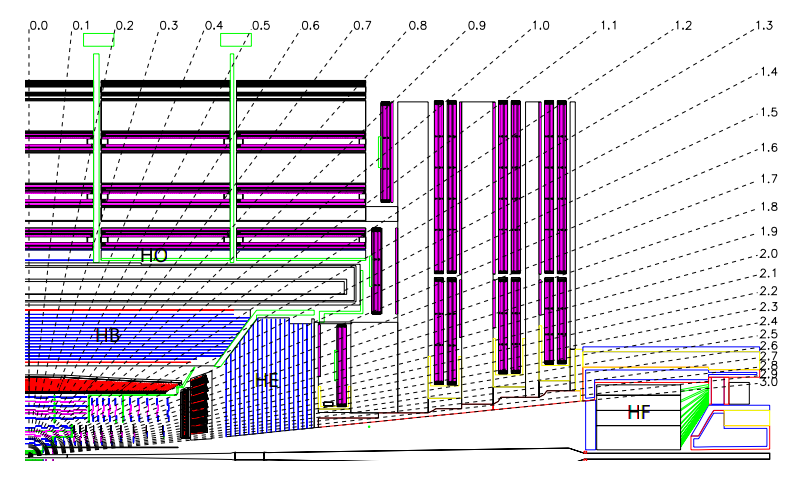
\includegraphics[width=1.0\textwidth]{detectorFigures/cms_hcal.png}
\caption[Schematic \crosssection of one quadrant of the HCAL, showing the arrangement of the various components of the \subdetector: The HB and HE surrounding the ECAL, with the HF at high $\eta$ and the HO just outside of the solenoid\quad\cite{CMSatLHC}.]{Schematic \crosssection of one quadrant of the HCAL, showing the arrangement of the various components of the \subdetector: The HB and HE surrounding the ECAL, with the HF at high $\eta$ and the HO just outside of the solenoid~\cite{CMSatLHC}.}
\label{fig:hcal}
\end{figure}

The minimum depth of the \HB is 5.8 radiation lengths, rising to 11.8 when the \HO is taken into account. In the endcaps, the depth is at least 10 radiation lengths~\cite{cmsHcal}. The resolution of the \HCAL system was measured in test beams of single pions~\cite{Abdullin:2009zz} and found to be:
\begin{equation}
\label{eq:HCALresol}
\left( \frac{\sigma}{E}\right) ^2= \left( \frac{94.3\%}{\sqrt{E}} \right)^2 + \left( \frac{8.4\%}{E} \right)^2.
\end{equation}

\subsection{Muon detectors}
\label{sec:cms:muondetector}

The solenoid is surrounded by the outermost \subdetector, the muon detector, which is built into and around the steel return yoke for the magnetic field.
The \CMS muon detection system consists of both endcap and barrel sections and is comprised of three types of detector: the \DTs in the barrel, the \CSCs in the endcaps, and the \RPCs in both barrel and endcaps. The muon chambers are all installed between the layers of the steel return yoke. The layout of the muon detectors can be seen in \Fig~\ref{fig:muonssystem}. All the muon detectors are gaseous detectors with a similar operational principle: as charged particles travel through a chamber, the gas contained within becomes ionised and the resulting electrons drift towards the detector's anode, which gives out an electric signal. 
\begin{figure}[h]
\centering
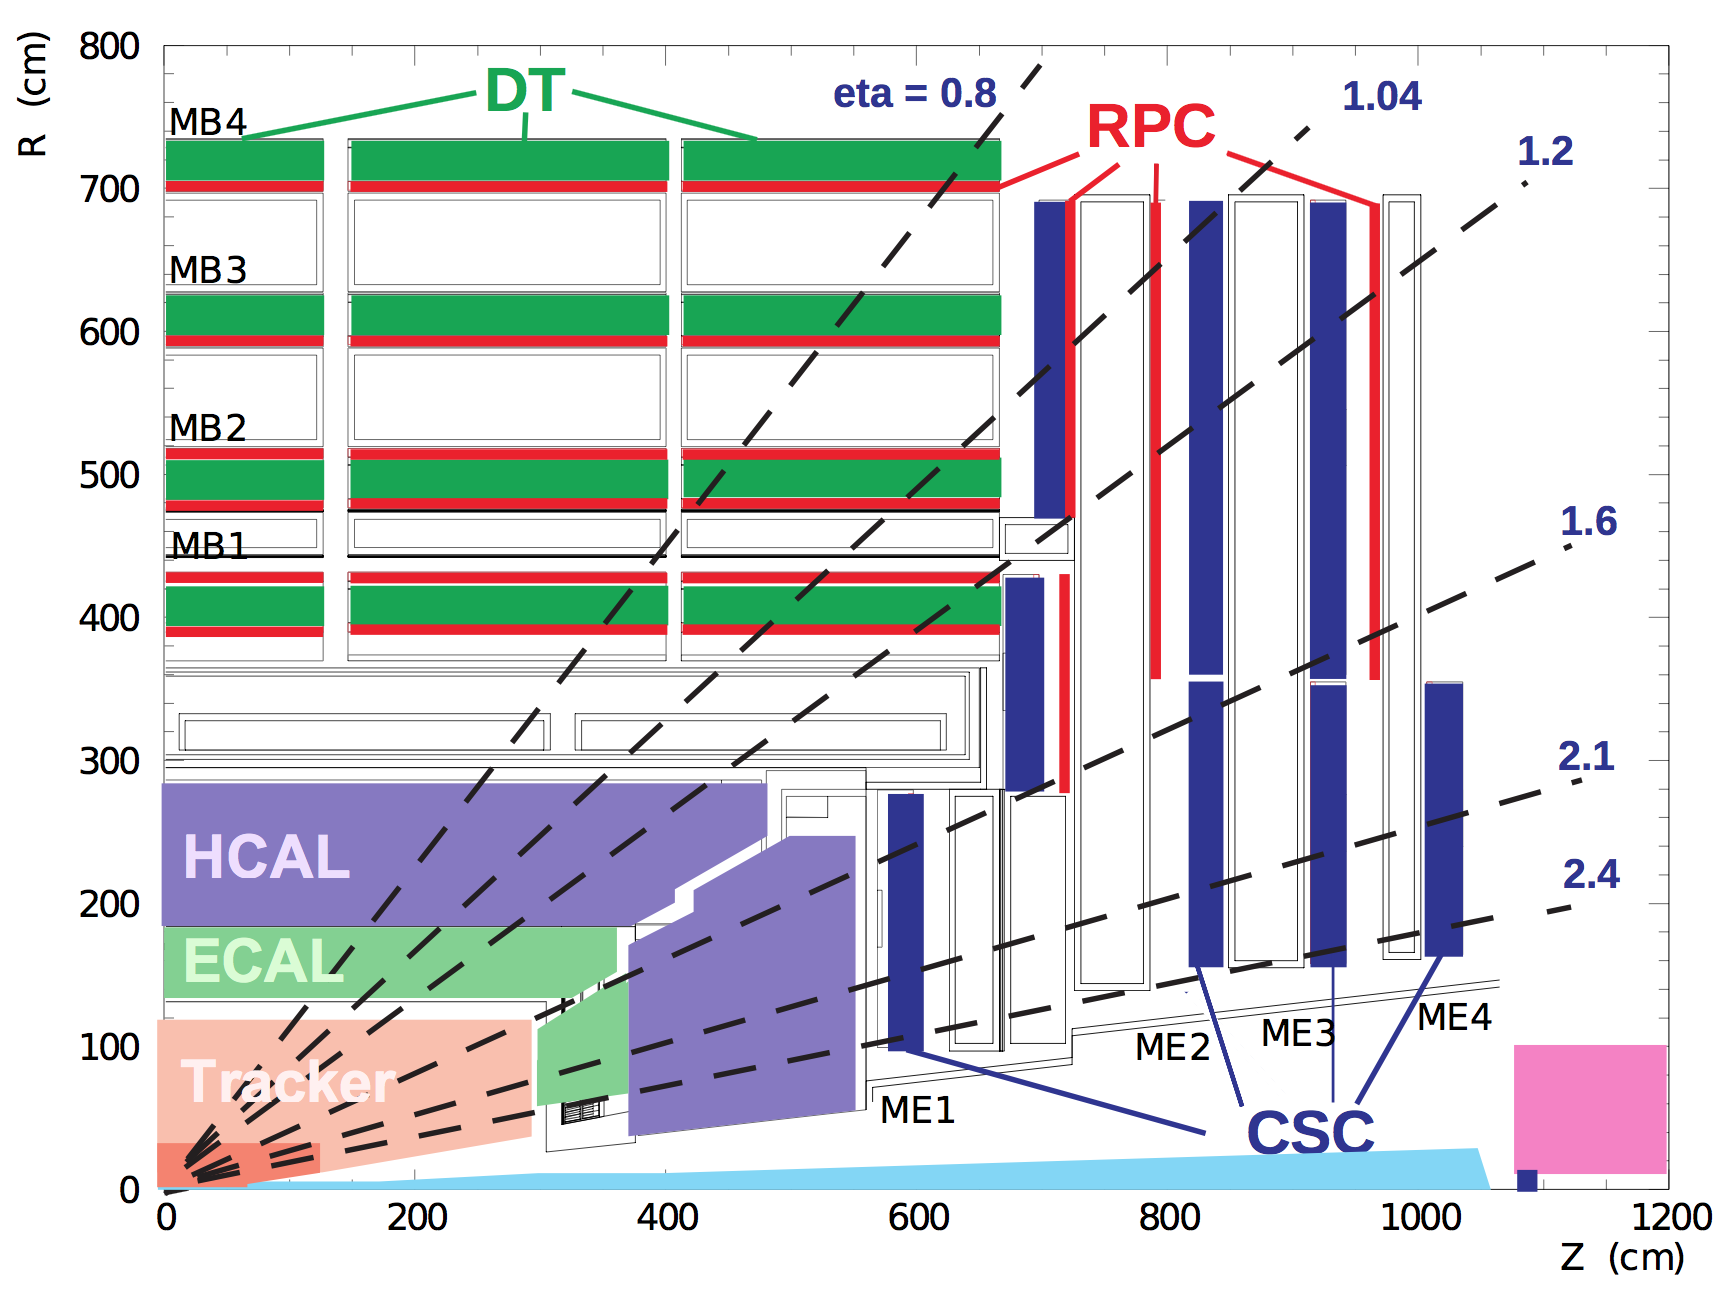
\includegraphics[width=1.0\textwidth]{detectorFigures/cmsMuonSystem.png}
\caption[Schematic \crosssection of one quadrant of the CMS muon detector, showing the arrangement of the various components of the sub-detector: The DTs in the barrel, and CSCs in the endcaps and the RPCs in both\quad\cite{MuonReco}.]{Schematic \crosssection of one quadrant of the CMS muon detector, showing the arrangement of the various components of the sub-detector: The DTs in the barrel, and CSCs in the endcaps and the RPCs in both~\cite{MuonReco}.}
\label{fig:muonssystem}
\end{figure}

 In the barrel section, the muon system is composed of four concentric layers of \DTs, which are wire chambers filled with a mixture of gaseous Ar and CO$_{2}$. Each DT station consists of twelve layers of wire chambers, with some having their wire oriented parallel to the beam axis and other perpendicular to it. This means that each DT is able to provide a position measurement in both the transverse and longitudinal planes, with 100\um resolution in each. The \DTs have coverage up to $|\eta|<1.3$. 

In the endcaps, the field is less uniform and the neutron fluences become much larger. The muon rate is also much higher than in the barrel. Therefore, a detection system with a faster response and more resistance to radiation is needed. The \CSCs, which are multi-wire chambers comprised of 6 anode wire planes interleaved among 7 cathode panels, satisfy this requirement. They are filled with a mixture of Ar, CO$_{2}$ and CF$_{4}$ gasses, and each station is also able to provide a measurement in both the longitudinal and transverse planes, with a spatial resolution around 85\um. There are four layers of \CSCs in each endcap, with coverage of $0.9<|\eta|<2.4$.

The final detector in the muon system is the array of \RPCs. These are double-gap chambers, and have a fast response with good timing resolution but worse position resolution than the \DTs or \CSCs. The \RPCs are used as a trigger, and can also be used to resolve ambiguities in tracking when there are multiple hits in a chamber. The \RPCs are installed in both the barrel and endcap sections, up to $|\eta|<1.6$~\cite{CMSatLHC,cmsMuon}. 

The transverse energy resolution for muons with \pT below 100\GeV is 1-6\% depending on their position within the detector~\cite{MuonReco}.

\subsection{Trigger and data processing}
\label{sec:cms:trigger}

During operation, bunch crossings occur at a rate of up to 40\MHz. Each instance where the data from a bunch crossing are saved by the detector is known as an event. The storage space taken up by an event is of the order of 1\MB. If \CMS were to keep all the information from each crossing, it would therefore need to save 40\TB of data per second, which is (at the time of writing) entirely impossible to store. Furthermore, the \CMS sub-detector electronics are designed to read out information at a rate of at most 100\kHz, so it is not possible to read out all the collision data either. Therefore, a vast reduction in the number of events selected to be saved is required. In reality, the vast majority of collisions are of no physics interest: many will be low-energy interactions of protons instead of head-on collisions, or will come from well-understood \SM processes. The strategy to reduce the number of selected events is to filter out the commonplace events and save only those which are of physics interest. This is achieved through the \CMS triggering system. The trigger is used to reduce the number of saved events by a factor of order $10^5$. This is achieved through two trigger levels: the \LI and the \HLT.

The \LI consists of programmable, custom-designed electronics. The \LI must reduce the number of output events by a factor of at least 400, since the maximum design bandwidth of the \subdetector electronics readout is 100\kHz. As collisions occur in the \CMS detector, each event is stored in a buffer. A very limited time, 3.2\us, is allocated to decide whether or not to save an event at the \LI. This must include the time taken to transmit the data from the sub-detectors to the \LI and return the decision to accept or not. The 3.2\us latency means that the buffer must be able to hold at least 128 bunch crossings. Due to bandwidth limitations and the short latency, decisions at the \LI are made based on very coarse data from the different detector subsystems individually. There no time to transmit or exploit their full granularity and resolution, or to use detailed correlations between different sub-detectors. The short amount of processing time available also prohibits the use of information from the tracker. Based on the coarse information available, the \LI runs a series of algorithms designed to identify events where processes of interest occur. In the case of a \LI accept, the full event data are transfered off the detector and passed to the \HLT~\cite{CMSatLHC}.

The \HLT consists of a farm of about 1000 commercially-available processors, which run basic reconstruction software and use the output to make a decision on which events to keep. The \HLT provides a further reduction the amount of data stored, decreasing it by a factor of about 100, down to an output of around 400\Hz. This is achieved using simplified versions of the full \CMS reconstruction software, with the full granularity of the information from the \CMS sub-detectors available, including from the tracker~\cite{CMSatLHC}.

Events passing the \HLT are then saved to disk and reconstructed using the full \CMS software for use in physics analyses.

